\subsection{Technologies, tools and frameworks}
Many different tools, libraries and frameworks were used in building the demonstration application. I will discuss the most important ones in greater detail.
\subsubsection{React}
React is a fast, declarative and efficient javascript library for creating web interfaces. It works around the concept of components. They are self-contained and composable blocks of code that encapsulates a part of user interface and its functionality. By putting together multiple small components it's possible to build complex user interfaces (UI). Components can be stateful or stateless.
The library provides a virtual-dom similar to the browsers document object model (DOM). They are both node trees that list elements together with attributes and content as objects and properties. Updating the dom is rather slow which is why the virtual-dom is useful for efficiency. It allows react to optimize DOM updates under the hood to only happen when it's necessary.

\subsubsection{Docker \& Containers}
Containers are self-contained pieces of code that can be run on any computer and operating system (OS). They contain the code and all of its necessary parts such as libraries, tools, and frameworks. They are similar to virtual machines but the main difference is in efficiency and application size. Containers are more efficient and smaller because they run on the same underlying kernel as the operating system as opposed to virtual machines which runs an entirely different OS.

Docker is tool that allows creating, running and managing containers. First we must create a dockerFile, which defines all the dependencies needed to run our code \ref{dockerFile}.

\begin{figure}[h!]
    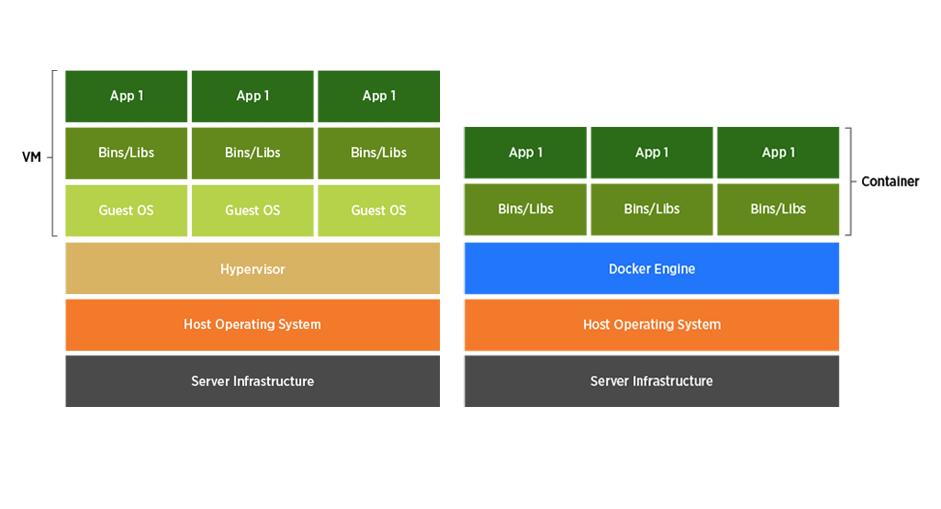
\includegraphics[scale=0.5]{containers-vs-vm-diagram}
    \caption{Container and virtual-machine comparison diagram}
\end{figure}

\subsubsection{Kubernetes}
Kubernetes is a container orchestration platform created by Google and open-sourced in 2014. It allows automation of deployment, scaling, and management of containerized applications. It groups the containers that make up a multi micro-service application into logical units for easy discovery and management. It's built with scalability in mind and provides other useful features such as load-balancing, logging, and monitoring. Kubernetes allows running containers in a cluster of physical and virtual computers called nodes. This is especially easy when using a cloud provider because of the vast availability of resources. 
I decided to use GKE, which is googles implementation of kubernetes in the cloud. This is in part due to their experience with running it in production environments used by millions of people. 

\subsubsection{Mongodb \& Mongoose}
MongoDB is an open source document oriented database, which stores data in json like format. Its characteristics include high availability, high performance, high flexibility and easy scaling. It stores data internally as BSON, a binary representation of json A collection is a schema-less entity which contains multiple documents and is the counterpart of a relational database table.

Mongoose is a javascript object data modelling library, that provides an easy to use interface for working with mongoDB. It provides an easy way to translate between javascript objects and mongoDB document representations. While being schema-less at database layer provides great flexibility, in a modern application we still need to enforce it at the application layer. This can be achieved with mongoose models and schemas. The schema much like in relational databases defines fields and their types. A model is just a wrapper around a schema. This model provides an extensive and flexible api for working with the underlying collections.

The application make uses a mongoDB atlas cloud instance with a separate database for each micro-service to store data. Due to the nature of mongoDB its possible too scale together with demand to more instances and shards.

\subsubsection{Keras}

Keras is a deep learning framework that provides an easy to use high level API. It provides efficient implementations of generally used layers, activations, loss functions and optimizers. The API is very intuitive and has a friendly implementation as its core principle. Furthermore, it is modular and easy to extend with custom functions and classes.
Keras wraps around a different number of low-level libraries called backends. These are Theano, Cognitive Toolkit, and TensorFlow. 
I have decided to use it with the tensorflow backend, because of its performance and ease of multi-gpu training (\citet{tensorflow2015-whitepaper}). 

\subsection{Micro-services}
The demo application follows a micro-services architecture composed of four applications \ref{architecture_diagram}. Each service has a specific role in the overall system. 

\begin{figure}[h!]
    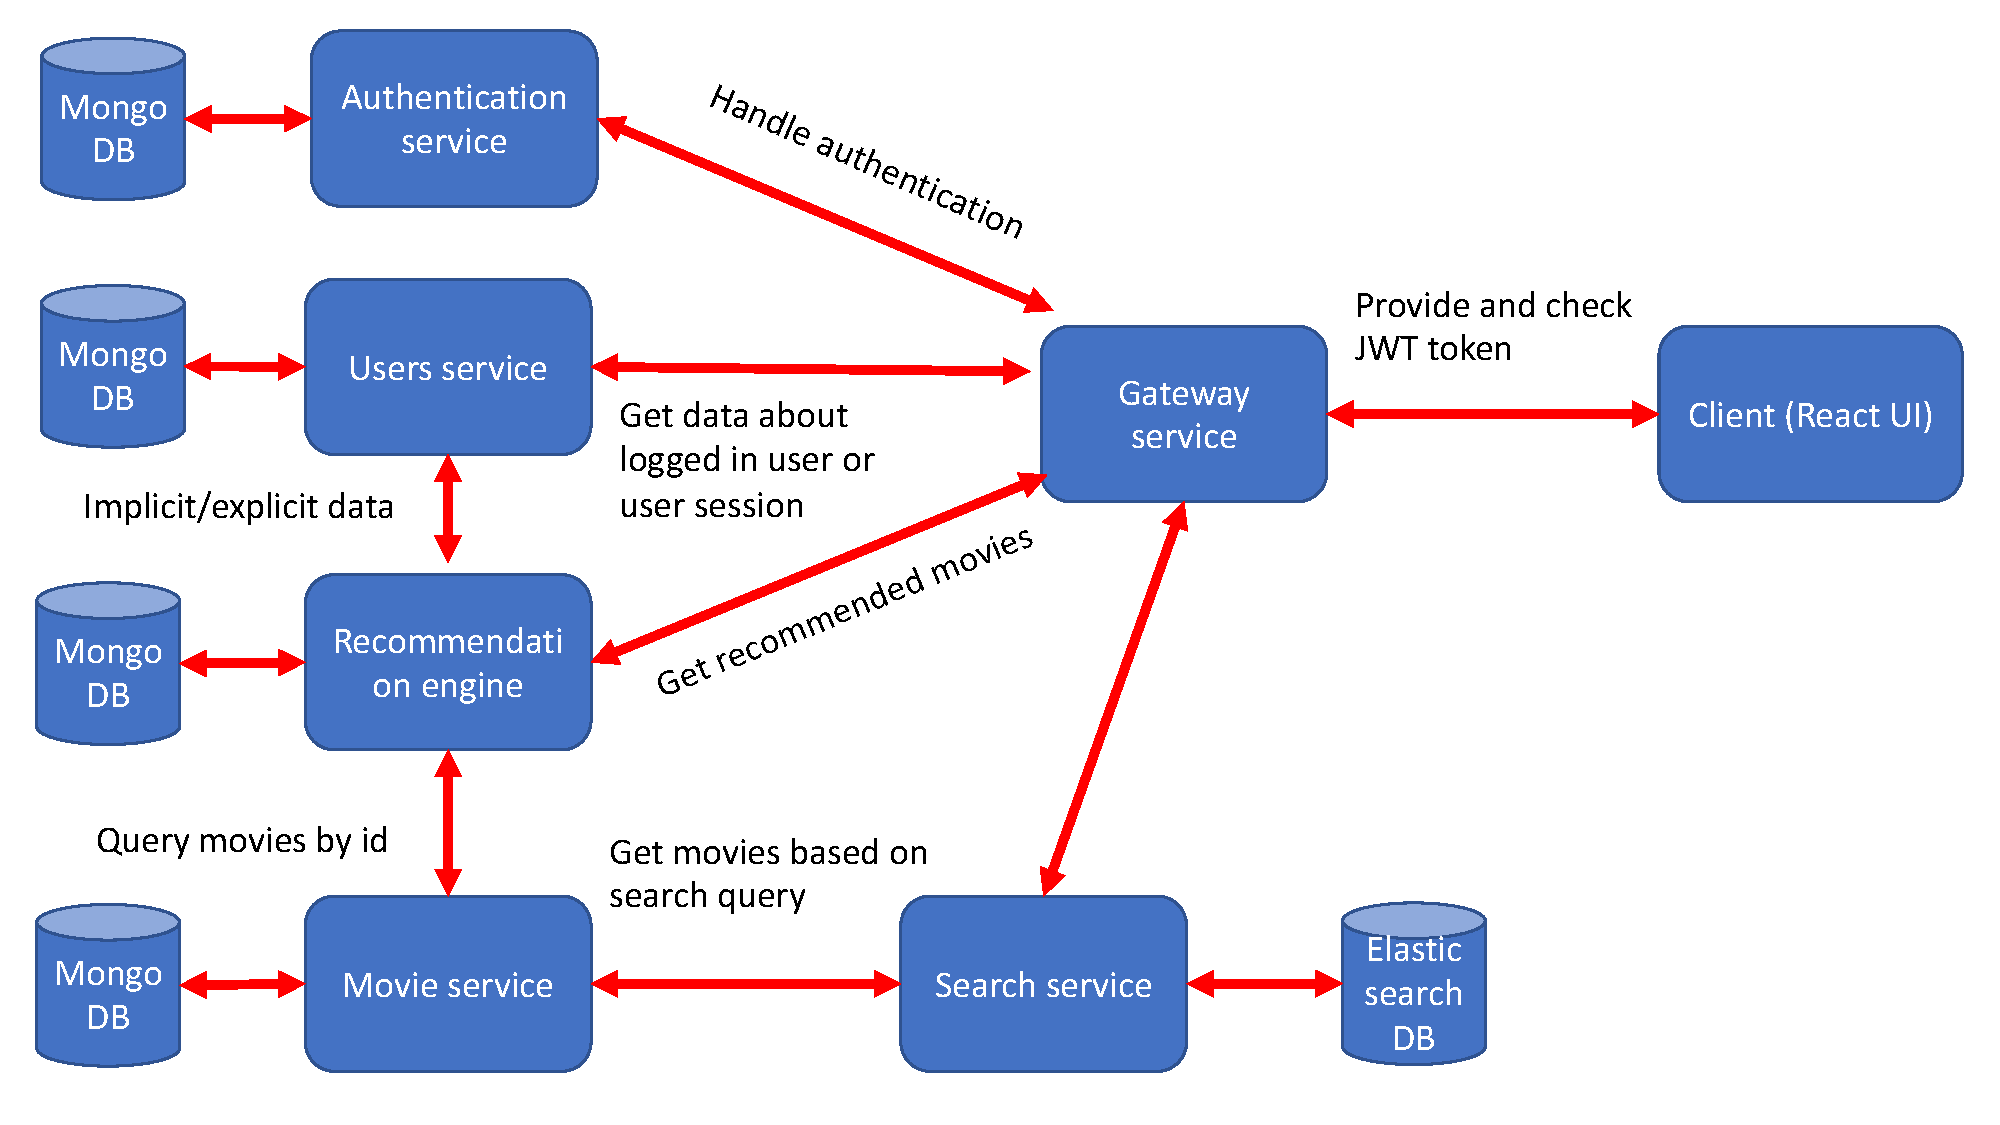
\includegraphics[scale=0.4]{architecture_diagram}
    \caption{Architecture diagram}
    \label{architecture_diagram}
\end{figure}

\begin{itemize}
    \item Gateway service is tasked with keeping track of user sessions and authentication.
    \item User service keeps track of user data including all their ratings.
    \item Movie service manages movies and all data related to them.
    \item Engine service manages the recommendations model, including retraining and serving.
\end{itemize}
The gateway exposes endpoints for login, signup and creation of initial session.
The movie service exposes endpoints for retrieving movies by id or search based on a query. In case of query retrieval it handles pagination of results.
The user service exposes endpoints for adding a new rating for a movie, updating a movie rating with a new value, getting all the ratings of a user.
The engine service exposes endpoints for retrieving top k recommendations of a certain user based on their id. Where k is a parameter in the request which allows serving different number of top recommendation results. It also exposes another endpoint which allows serving recommendations from a subset of the movies as defined by the search query results described in the movie service api. 


\subsection{Web application}
The demo application is created with ease of use in mind. It does not require creation of an account and instead uses the gateway service to provide a signed json-web-token (JWT) to identify users. This token is held in the browser local storage of each user. The frontend uses this token in authentication headers when making request to the backend services. 
If at any point later a user decides to create an account, the system automatically handles it by merging the current data with the newly created account \ref{user_flow}.
\begin{figure}[h!]
    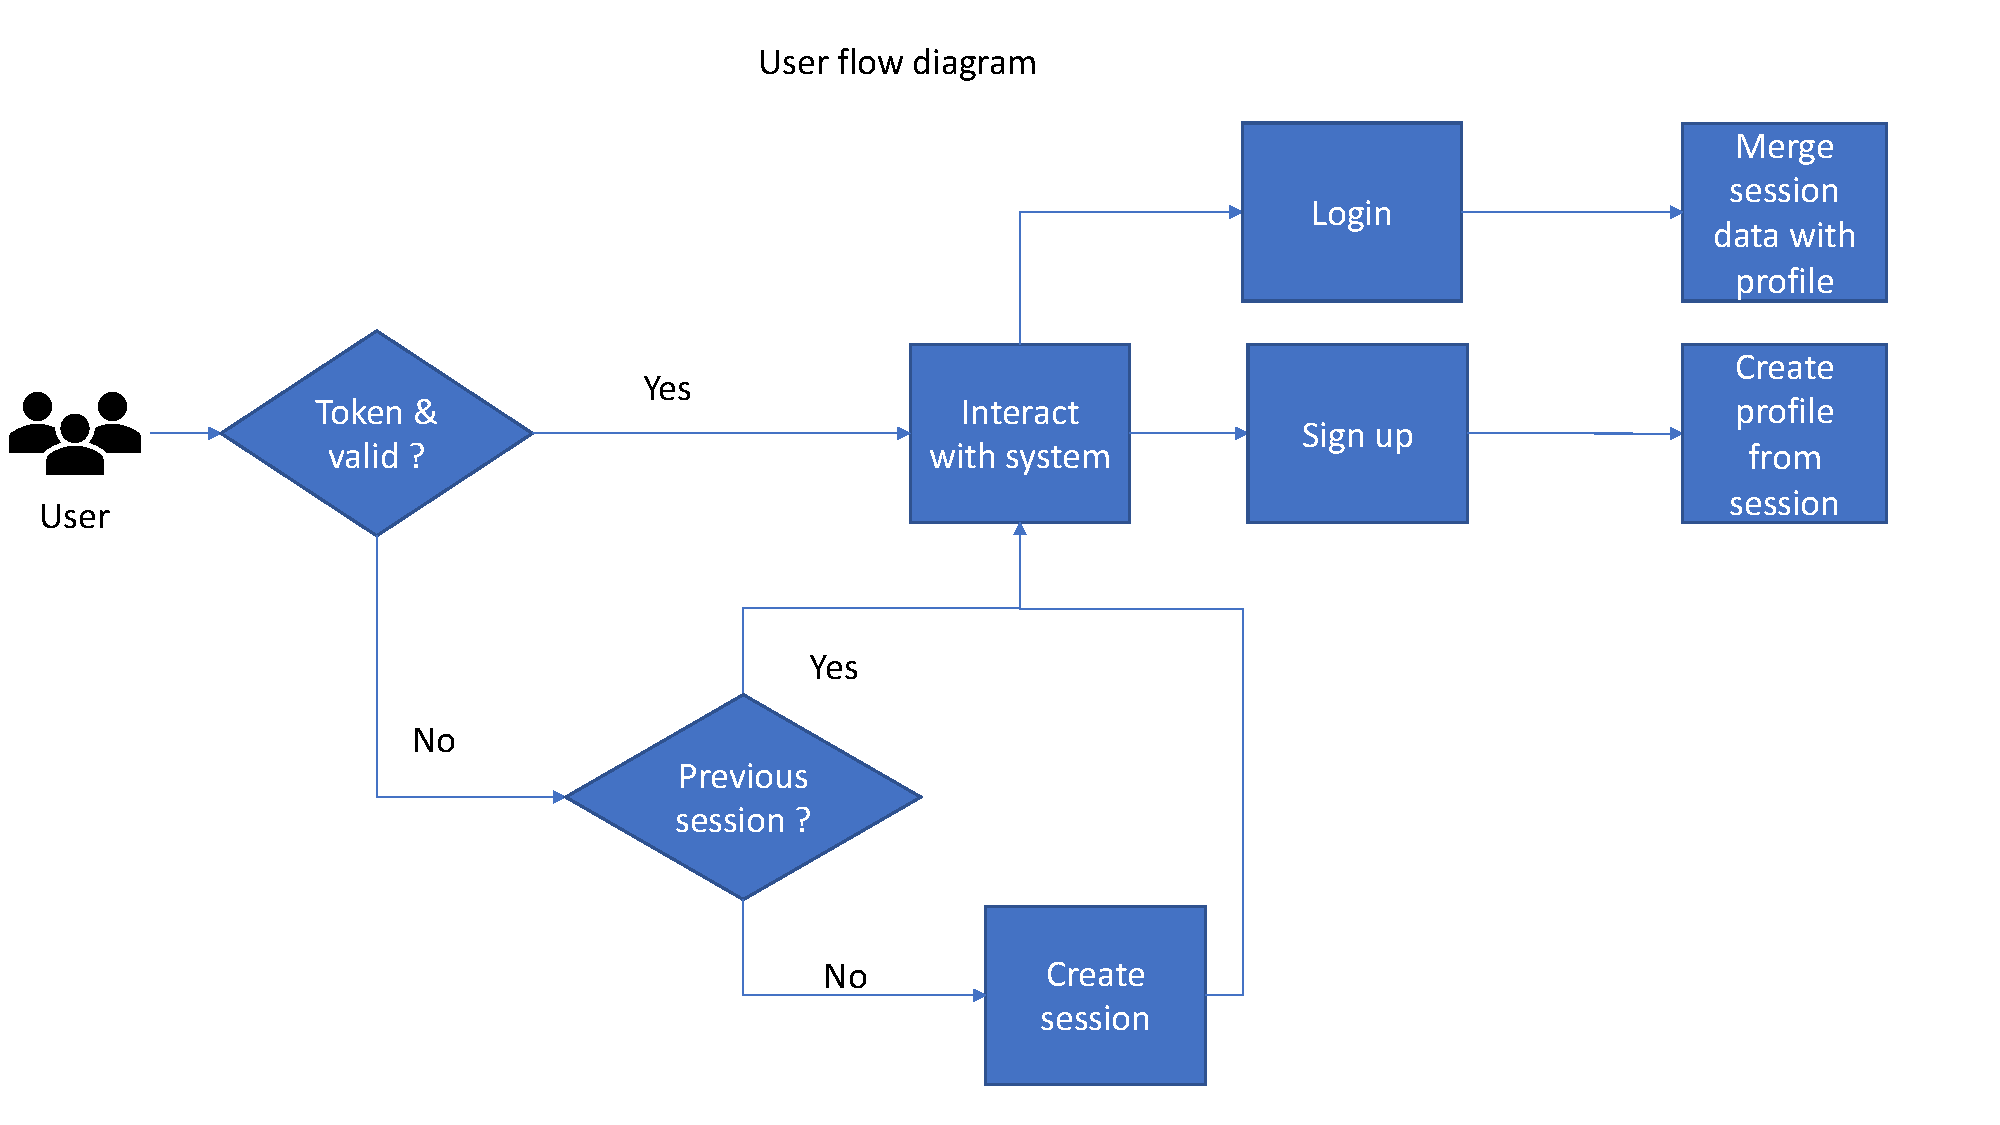
\includegraphics[scale=0.4]{user_flow_diagram}
    \caption{User flow diagram}
    \label{user_flow}
\end{figure}

The demo app displays a list of movies that can be rated on scale of 0.5 to 5 in 0.5 increments. The app was built with user interface responsiveness in mind from the beginning, this means the layout is self-adjusting to display nicely on different size displays and also on mobile.

\begin{figure}[h!]
    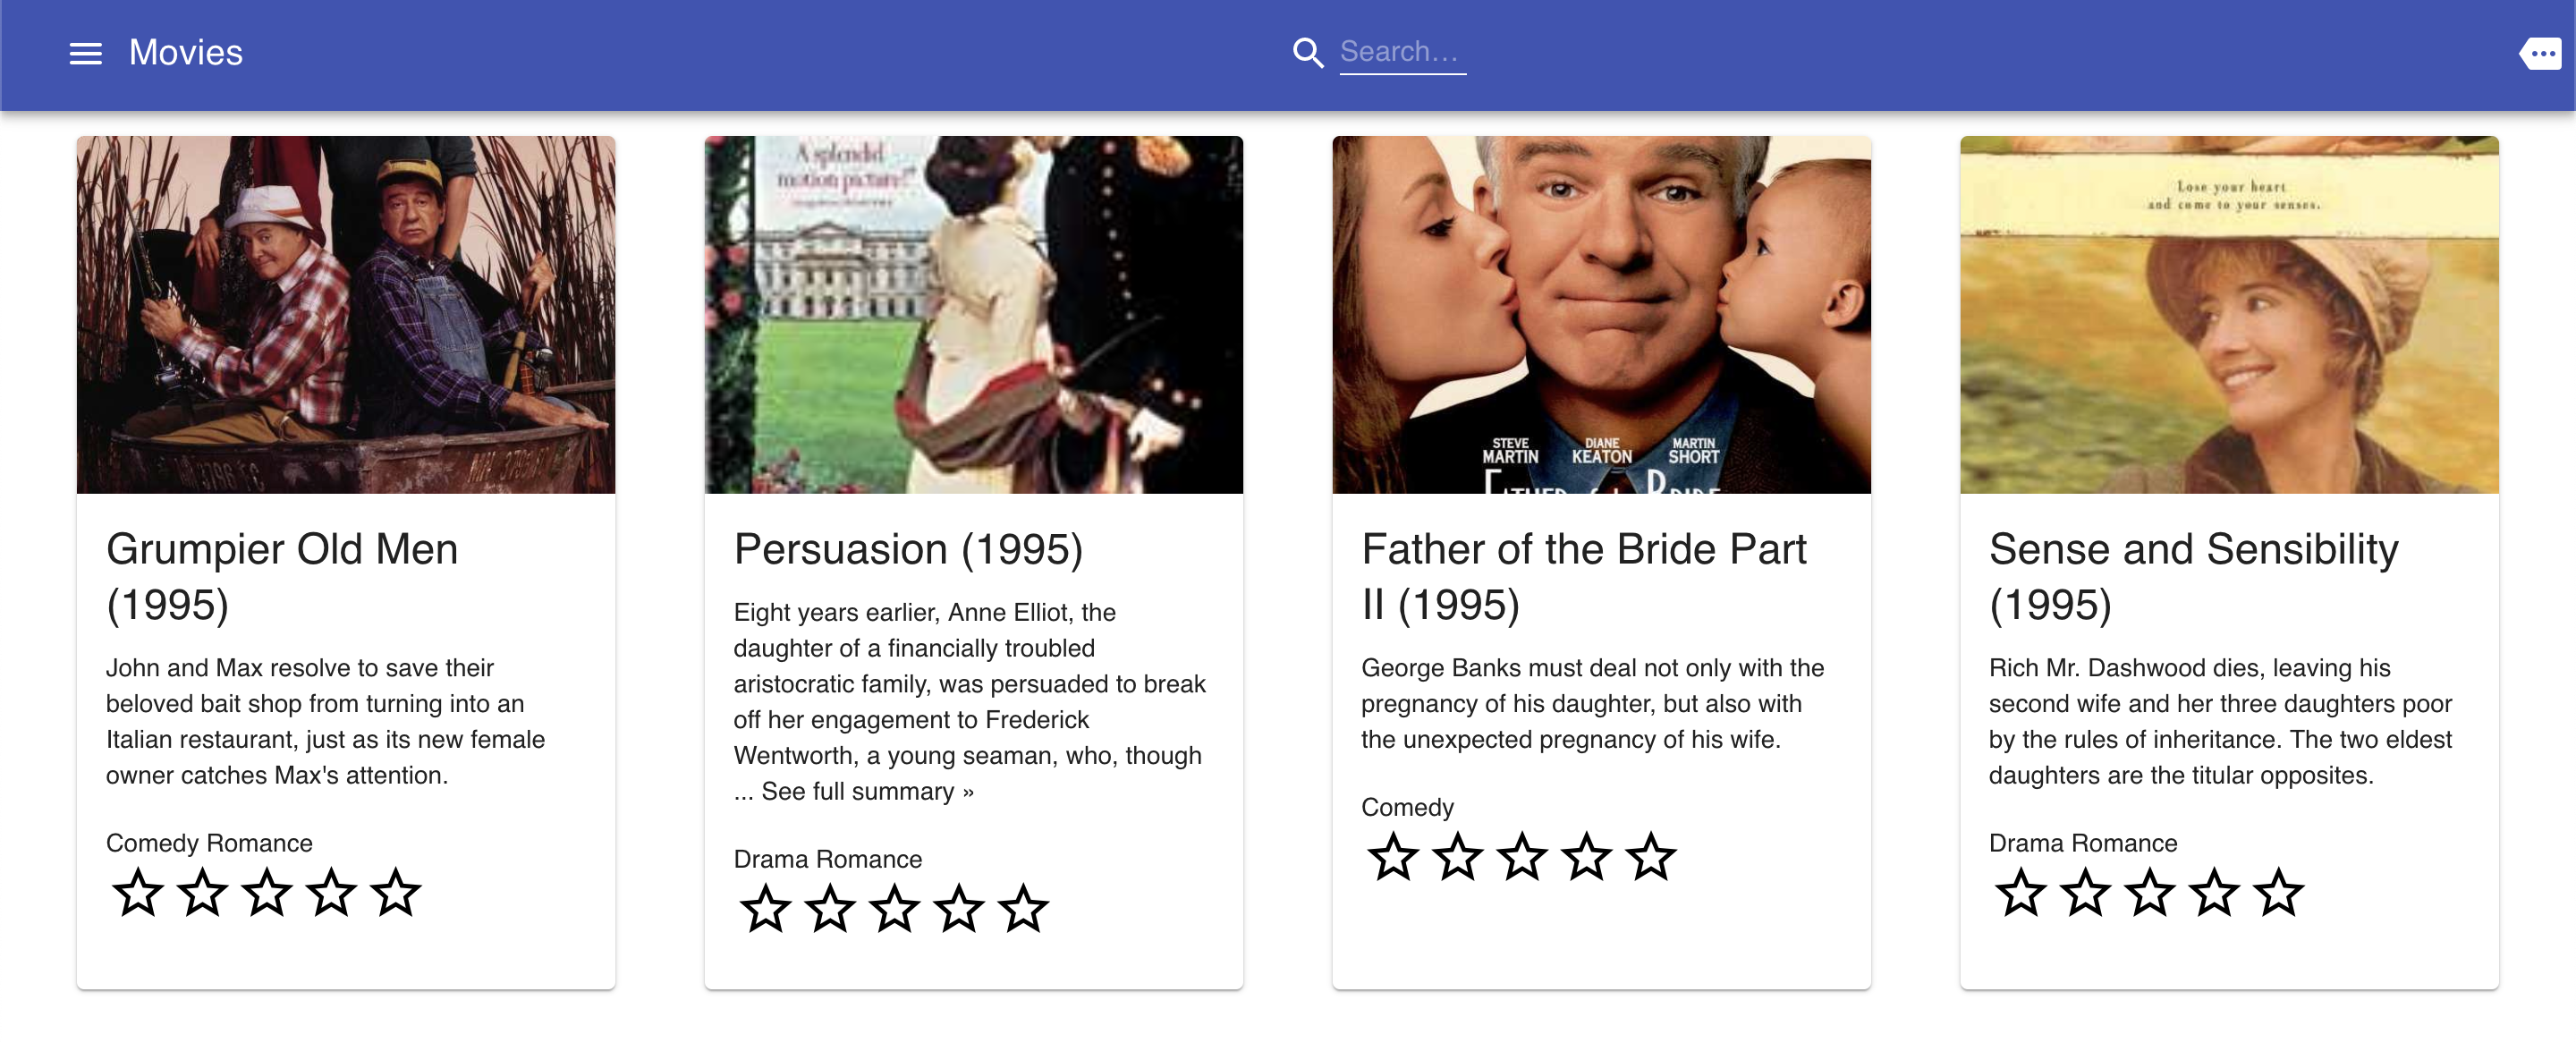
\includegraphics[scale=0.3]{movie_list}
    \caption{Movie list desktop}
    \label{movie_list}
\end{figure}

\begin{figure}[h!]
    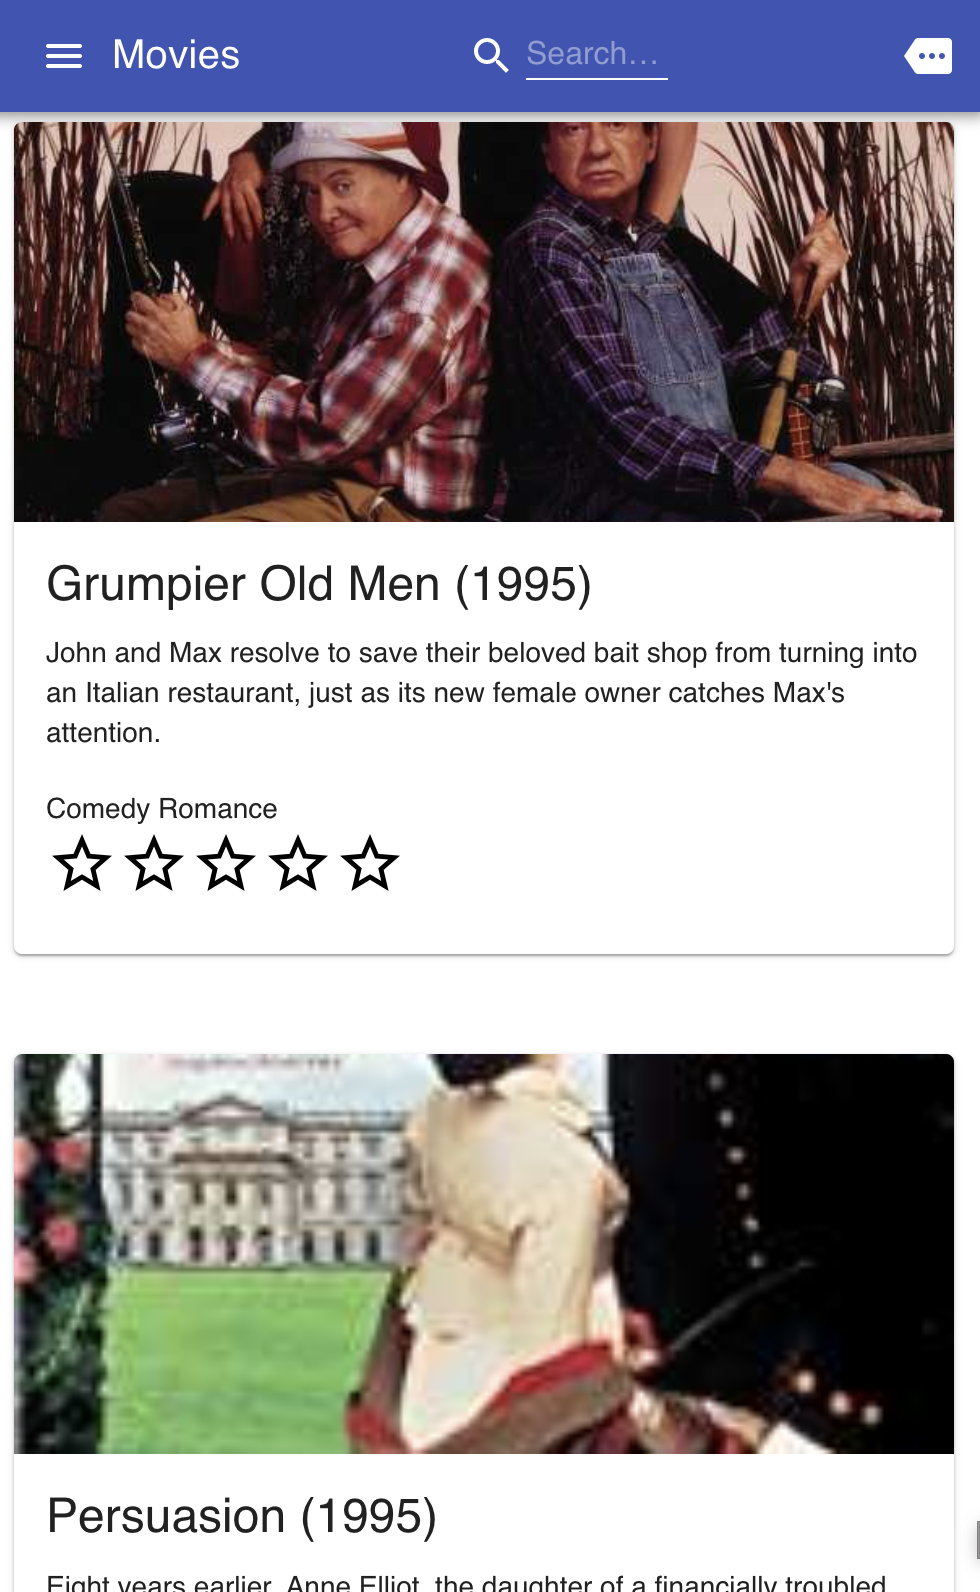
\includegraphics[scale=0.4]{movie_list_mobile}
    \caption{Movie list mobile}
    \label{movie_list}
\end{figure}